\documentclass{beamer}
\usepackage[utf8]{inputenc}
\usepackage[english]{babel}

\usepackage{graphicx}
\usepackage{wrapfig}

\usepackage{mathtools}
\usepackage{commath}
% \usepackage{amscmd}

\mode<presentation>{\usetheme{Warsaw}
}

\newcommand*{\Dt}{\Delta{}t}

\title[Simulating the Schrödinger Equation with Finite Elements]{Schrödinger FEM}

\author{Bernd Schwarzenbacher}
\institute[KTH]
{Stockholm \\
\medskip
}
\date{\today}

\begin{document}

\begin{frame}
  \frametitle{Time-Dependent Schrödinger Equation}
\[ -\frac{\hbar^2}{2m} \nabla^2 \Psi + V \Psi = i \hbar \frac{\partial\Psi}{\partial{}t}\]
\pause
\[\Bigg\downarrow\]
\[A u = M \frac{\partial{}u}{\partial{}t}\]

\begin{wrapfigure}[1]{r}{0.2\textwidth}
  \vspace{-30pt}
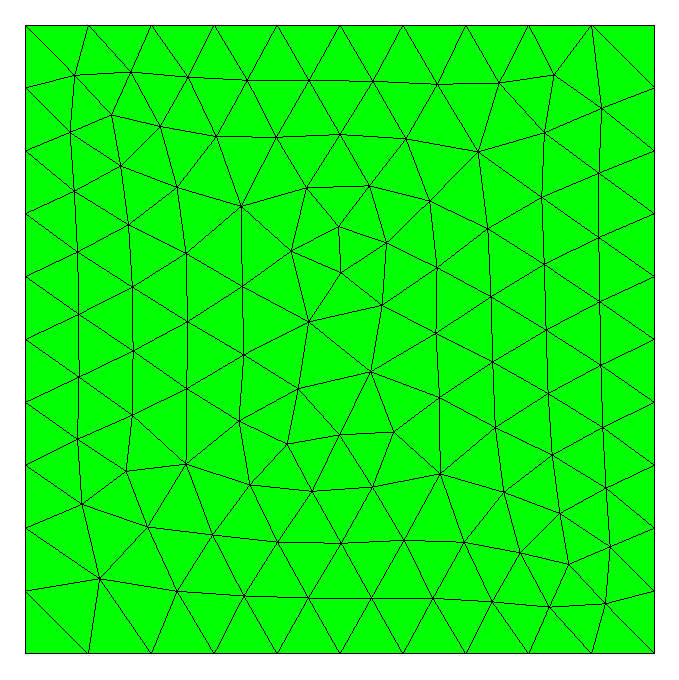
\includegraphics[width=\linewidth]{mesh.png}
\end{wrapfigure}
spatial discretization: Finite Element Method 
\end{frame}

\begin{frame}
  \frametitle{Time-Stepping}
\[A u = M \frac{\partial{}u}{\partial{}t}\]
need Isometry: $\norm{u_{n+1}} = \norm{u_n}$

Crank-Nicolson method, trapezoidal rule:
\[ \frac{\Dt}{2} (A u_{n+1} + A u_{n}) = M (u_{n+1} - u_n) \]
\pause
\[ u_{n+1} =  u_n +  \Dt \left( \frac{\Dt}{2}A - M \right)^{-1} A u_n\]
\end{frame}

\begin{frame}
  \frametitle{Implementation}
spatial discretization:
\[A u = M \frac{\partial{}u}{\partial{}t}\]
time-stepping:
\[ u_{n+1} =  u_n +  \Dt \left( \frac{\Dt}{2}A - M \right)^{-1} A u_n\]
\pause
\begin{wrapfigure}{r}{0.3\textwidth}
\begin{center}
  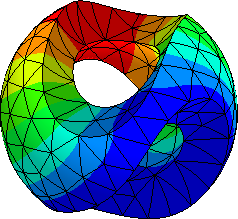
\includegraphics[width=0.4\linewidth]{logo-col-med2.png}
  \url{ngsolve.org}
\end{center}
\end{wrapfigure}
Netgen/NGSolve:
\begin{itemize}
 \item Python scripting \& C++ back end
 \item spatial discretization
 \item Inversion - computational intensive
\end{itemize}

\end{frame}

\end{document}